% !TeX spellcheck = en_GB
% !TeX encoding = UTF-8
\documentclass[8pt]{beamer}

 \usepackage[utf8]{inputenc}                                                     
 \usetheme[block=fill,progressbar=foot,background=light]{metropolis}                                                               
%  \usecolortheme{crane}                                                       
  %\useinnertheme{circles}                                                         
  \usepackage[english]{babel}                                                     
  \usepackage{csquotes}                                                           
  \usepackage[T1]{fontenc}                                                        
  \usepackage{booktabs}                                                       \usepackage{pgfgantt}
  \usepackage{pifont}
  \usepackage{adfbullets}
  \usepackage{enumitem}
  \usepackage{amsmath}   
  \usepackage{tikz}
  \usepackage{amssymb}
  \usepackage{amsfonts}
  \usepackage{mathrsfs}   
  \usepackage{graphicx}
  \usepackage{adjustbox}
  \usepackage{varioref}
  \usepackage{probsoln}
  \usepackage{attachfile2}
  \usepackage{pgfplots}
\pgfplotsset{compat=newest}
  \usepackage[style=authoryear,backref=true]{biblatex}
 \usepackage[]{hyperref} 
  \graphicspath{{Graphics/}}
  \usepackage{multirow,array}
  \addbibresource{../Everything.bib}
  \usepackage{colortbl}
  \definecolor{aa}{RGB}{255, 124, 0}
  \definecolor{cc}{RGB}{230, 230, 230}    
  %\setbeamercolor{palette tertiary}{fg=aa,bg=cc}
  %\setbeamercolor{structure}{fg=cc}
  %\setbeamercolor{alerted text}{fg=red}
  
  %Information to be included in the title page:
  
  \usebackgroundtemplate{%
  \tikz[overlay,remember picture]{\node[scale=80,opacity=0.03, at=(current page.south east)] {\adfbullet{9}};}}
  
  \author[]{T. Bretschneider}
  
  \date[\today]{\today}

\usepackage{comment}
\usepackage{varwidth}

\newcommand{\mat}[4]{\left(\begin{array}{cc} #1 & #2 \\ #3 & #4 \\ \end{array}\right)}
\newcommand{\Q}{\mathbb{Q}}
\newcommand{\R}{\mathbb{R}}
\newcommand{\Z}{\mathbb{Z}}
\newcommand{\sol}[2][+]{
	\tikz[baseline]{\node[color=aa,fill=cc,rectangle,draw,anchor=base] {  {\onslide<#1->{#2}}  };}
}

\usetikzlibrary{positioning}
\usetikzlibrary{tikzmark}
\usetikzlibrary{shadings}
\usetikzlibrary{through}


\def\height{0.8cm}
\def\width{1.2cm}

		\newcommand{\keynode}[6]{\node[minimum height=\height,minimum width=\width,draw,rectangle,color=aa,fill=cc] (#3) at (#1,#2) {};
	\node[rectangle,minimum height=\height/2,minimum width=\width,above,color=aa] at (#3) {#3};
	\node[draw,rectangle,minimum height=\height/2,minimum width=\width/3,below,color=aa,fill=cc,inner sep =0cm] at (#3) {\footnotesize#4};
	\node[draw,rectangle,minimum height=\height/2,minimum width=\width/3,below,xshift=\height/2,color=aa,fill=cc,inner sep=0cm] at (#3) {\footnotesize#5};
	\node[draw,rectangle,minimum height=\height/2,minimum width=\width/3,below,xshift=-\height/2,color=aa,fill=cc,inner sep=0cm] at (#3) {\footnotesize#6}; }

\newenvironment{gantt}[3]{\begin{ganttchart}[#1,bar height=.6,bar top shift=.2,title/.style=  {draw=none},y unit chart=0.6cm,y unit title = 0.6cm,include title in canvas=false,group/.append style={draw=black,dashed},bar/.append style={fill=aa},inline,hgrid=true,Float1/.style={bar/.append style={fill=none,dashed},bar height=.8,bar top shift=0.1}]{#2}{#3}}{\end{ganttchart}}

\newenvironment{nicetable}[1]{\setlength\arrayrulewidth{0.5mm}
			\arrayrulecolor{white}
			\begin{tabular}{#1}}{\end{tabular}}
		
\setlist[itemize,1]{label={\color{aa}\huge\adfbullet{9}}}
\setlist[itemize, 2]{label={\color{aa}\large\adfbullet{9}}}

\newcommand\reshist{}
\def\reshist(#1)#2(#3)#4(#5)%
{\draw (axis cs:#1) rectangle (axis cs:#3) node [midway] {#5};}







  \title[Discrete]{{\color{aa}\Huge\adfbullet{9}}AL FM Discrete}
  \subtitle{Gantt Charts and Resource Histograms, \textattachfile{GanttChartsandResourceHistograms.tex}{(TeX)}}

\begin{document}

\setlength{\abovedisplayskip}{0pt}
\setlength{\belowdisplayskip}{0pt}
\setlength{\abovedisplayshortskip}{0pt}
\setlength{\belowdisplayshortskip}{0pt}


\frame{\titlepage}

\begin{frame}[shrink=5]{Gantt Chart}
	\begin{definition}
		A \textbf{Gantt Chart} (also know as a \textbf{Cascade Chart} has the following features:
		\begin{itemize}
			\item Activities are represented by horizontal bars, beginning at their earliest start times.
			\item Critical activities are drawn on a single line and all other activities should be drawn on an separate line.
			\item the bars are divided into two parts:
				\begin{itemize}
					\item The first is the duration of the activity and is usually shaded solidly
					\item The second is the float which is usually given a dotted border
						
				\end{itemize}
			\item Sometimes the number of workers required for each activity may be shown on the bar.
		\end{itemize}
	\end{definition}

\centering
	\begin{gantt}{vgrid}{0}{17}
	\gantttitlelist{0,...,17}{1} \\
	\ganttbar{C}{0}{5} 
	\ganttbar{E}{5}{13}
	\ganttbar{G}{13}{17} \\
	\ganttbar{A}{0}{2} 
	\ganttbar[Float1]{}{0}{7} \\
	\ganttbar{B}{0}{3} 
	\ganttbar[Float1]{}{0}{7} \\
	\ganttbar{D}{3}{9}
	\ganttbar[Float1]{}{3}{13} \\
	\ganttbar{F}{5}{7}
	\ganttbar[Float1]{}{5}{17} 
\end{gantt}

\end{frame}

\begin{frame}{Example}
	\begin{columns}
		\begin{column}{.5\textwidth}
	You might have to draw an Activity Network so that you know which activities are on the critical path and the earliest start and slack for the others. For smaller problems though you might be able to do this by inspection.
\end{column}
	\begin{column}{.5\textwidth}
	\begin{center}
	\colorbox{cc}{
		\begin{nicetable}{cc>{\centering\arraybackslash}m{1.7cm}}
			Task & Duration & Immediate predecessors \\
			\hline
			A & 3 &  \\
			B & 4 &  \\
			C & 6 & \\
			D & 5 & A \\
			E & 1 & B \\
			F & 6 & B \\
			G & 7 & C,D,E \\ 	
\end{nicetable}}
\end{center}
\end{column}
\end{columns}
	\begin{gantt}{vgrid}{0}{15}
	\gantttitlelist{0,...,15}{1} \\
	\ganttbar{A}{0}{3} 
	\ganttbar{D}{3}{8}
	\ganttbar{G}{8}{15} \\
	\ganttbar{B}{0}{4} 
	\ganttbar[Float1]{}{0}{7} \\
	\ganttbar{C}{0}{6} 
	\ganttbar[Float1]{}{0}{8} \\
	\ganttbar{E}{4}{5}
	\ganttbar[Float1]{}{4}{8} \\
	\ganttbar{F}{4}{10}
	\ganttbar[Float1]{}{4}{15} 
\end{gantt}

\end{frame}

\begin{frame}{Interpreting a Gantt Chart}
	\begin{problem}
		\begin{minipage}{.4\linewidth}
		The following Gantt chart represents a project. It transpires that A and B both require use of the same equipment. Can the project still be completed in 15 hours. Give your reasons.
	\end{minipage}%
	\begin{minipage}{.6\linewidth}
		\centering
		\adjustbox{max width=5cm}{
			\begin{gantt}{canvas/.append style={fill opacity=0},vgrid}{1}{15}
	\gantttitlelist{1,...,15}{1} \\
	\ganttbar{A}{1}{3} 
	\ganttbar{D}{4}{8}
	\ganttbar{G}{9}{15} \\
	\ganttbar{B}{1}{4} 
	\ganttbar[Float1]{}{1}{7} \\
	\ganttbar{C}{1}{6} 
	\ganttbar[Float1]{}{1}{8} \\
	\ganttbar{E}{5}{5}
	\ganttbar[Float1]{}{5}{8} \\
	\ganttbar{F}{5}{10}
	\ganttbar[Float1]{}{5}{15} 
\end{gantt}}
\end{minipage}
	\end{problem}

\begin{solution}<2->
	\begin{minipage}{.5\linewidth}
	A and B are originally both scheduled at the same time. Since A is critical, moving A would result in a delay. So consider moving B. This means that E and F must also move.

The new cascade diagram shows that moving B so that it starts after A ends, and moving E and F so that they still start after B ends, so the project can still be completed in 15 hours.
\end{minipage}%
\begin{minipage}{.5\linewidth}
		\centering
		\adjustbox{max width=5cm}{
			\begin{gantt}{canvas/.append style={fill opacity=0},vgrid}{1}{15}
	\gantttitlelist{1,...,15}{1} \\
	\ganttbar{A}{1}{3} 
	\ganttbar{D}{4}{8}
	\ganttbar{G}{9}{15} \\
	\ganttbar{B}{4}{7} 
	\ganttbar[Float1]{}{1}{7} \\
	\ganttbar{C}{1}{6} 
	\ganttbar[Float1]{}{1}{8} \\
	\ganttbar{E}{8}{8}
	\ganttbar[Float1]{}{5}{8} \\
	\ganttbar{F}{8}{13}
	\ganttbar[Float1]{}{5}{15} 
\end{gantt}}
\end{minipage}
\end{solution}


\end{frame}


\begin{frame}{Interpreting a Gantt Chart}
	\begin{problem}
		\begin{minipage}{.5\linewidth}
The following Gantt chart represents a project. It now transpires that A and C must be done by a qualified person and there is only one available. Can the project still be completed in 15 hours. Give your reasons.
\end{minipage}%
\begin{minipage}{.5\linewidth}
		\centering
		\adjustbox{max width=5cm}{
			\begin{gantt}{canvas/.append style={fill opacity=0},vgrid}{1}{15}
	\gantttitlelist{1,...,15}{1} \\
	\ganttbar{A}{1}{3} 
	\ganttbar{D}{4}{8}
	\ganttbar{G}{9}{15} \\
	\ganttbar{B}{1}{4} 
	\ganttbar[Float1]{}{1}{7} \\
	\ganttbar{C}{1}{6} 
	\ganttbar[Float1]{}{1}{8} \\
	\ganttbar{E}{5}{5}
	\ganttbar[Float1]{}{5}{8} \\
	\ganttbar{F}{5}{10}
	\ganttbar[Float1]{}{5}{15} 
\end{gantt}}
\end{minipage}
	\end{problem}

\begin{solution}<2->
	\begin{minipage}{.5\linewidth}
	A and C are currently scheduled together. Again, as A is a critical activity, it is probably better to move C. Note that G depends on C.

	In this case, C only has 2 hours of float so moving it by 3 hours means that G is moved by 1 hour. So the whole project is delayed by 1 hour.

	\alert<3>{Notice that in the situation above, the critical path has changed. It is now ACG.}
\end{minipage}%
\begin{minipage}{.5\linewidth}
		\centering
		\adjustbox{max width=5cm}{
			\begin{gantt}{canvas/.append style={fill opacity=0},vgrid}{1}{16}
	\gantttitlelist{1,...,16}{1} \\
	\ganttbar{A}{1}{3} 
	\ganttbar{D}{4}{8}
	\ganttbar{G}{10}{16} \\
	\ganttbar{B}{1}{4} 
	\ganttbar[Float1]{}{1}{7} \\
	\ganttbar{C}{4}{9} 
	\ganttbar[Float1]{}{1}{8} \\
	\ganttbar{E}{5}{5}
	\ganttbar[Float1]{}{5}{8} \\
	\ganttbar{F}{5}{10}
	\ganttbar[Float1]{}{5}{15} 
\end{gantt}}

\end{minipage}
\end{solution}


\end{frame}

\begin{frame}[shrink=5]{Resource Histograms}
	\begin{definition}
		A \textbf{resource histogram} is based on the Gantt chart but it also shows the number of workers required at each time.
	\end{definition}

	\begin{columns}
	\begin{column}{.6\linewidth}
	\begin{center}
		\adjustbox{max width=\linewidth}{
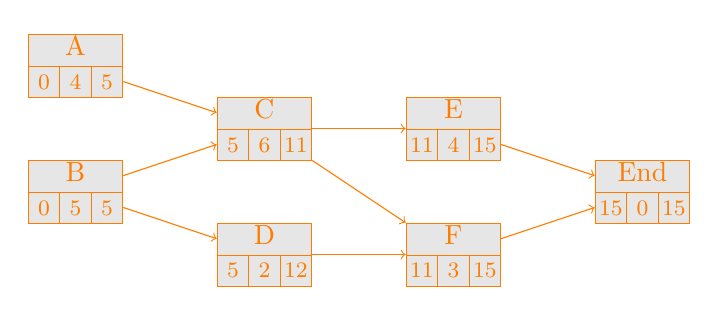
\begin{tikzpicture}
\keynode{0}{0}{A}{4}{5}{0}
\keynode{0}{-2*\height}{B}{5}{5}{0}
\keynode{2*\width}{-\height}{C}{6}{11}{5}
\keynode{2*\width}{-3*\height}{D}{2}{12}{5}
\keynode{4*\width}{-\height}{E}{4}{15}{11}
\keynode{4*\width}{-3*\height}{F}{3}{15}{11}
\keynode{6*\width}{-2*\height}{End}{0}{15}{15}

\draw[->,color=aa] (A) --  (C);
\draw[->,color=aa] (B) --  (C);
\draw[->,color=aa] (B) --  (D);
\draw[->,color=aa] (C) --  (E);
\draw[->,color=aa] (C) --  (F);
\draw[->,color=aa] (D) --  (F);
\draw[->,color=aa] (E) --  (End);
\draw[->,color=aa] (F) --  (End);
\end{tikzpicture}}

\end{center}
	\end{column}
	\begin{column}{.4\linewidth}
		\centering
		\adjustbox{max width=\linewidth}{
\begin{gantt}{vgrid}{1}{15}
	\gantttitlelist{1,...,15}{1} \\
	\ganttbar{B}{1}{5} 
	\ganttbar{C}{6}{11}
	\ganttbar{E}{12}{15} \\
	\ganttbar{A}{1}{4} 
	\ganttbar[Float1]{}{1}{5} \\
	\ganttbar{D}{6}{7} 
	\ganttbar[Float1]{}{6}{12} \\
	\ganttbar{F}{12}{14}
	\ganttbar[Float1]{}{12}{15} 
\end{gantt}}
	\end{column}
	\end{columns}
	

\begin{problem}
	Now also suppose that the activities require the following number of workers: 

	A:2, B:3, C:1, D:5, E:2, F:4
\end{problem}


\begin{solution}<2->
	\begin{center}
	\begin{tikzpicture}
					\begin{axis}[mlineplot,width=6cm,height=3cm,
						xmin= 0, xmax= 15,
						ymin= 0, ymax = 8,
						axis lines = middle,
					]
					\draw (axis cs:0,0) rectangle (axis cs:4,2) node[midway] {A};
					\reshist(0,2) (4,5) (B)
					\reshist(4,0) (5,3) (B)
				\reshist(5,0) (11,1) (C)
			\reshist(5,1) (7,6) (D)
		\reshist(11,0) (15,2) (E)
		\reshist(11,2) (14,6) (F)
					\end{axis}
				\end{tikzpicture}
			\end{center}
\end{solution}

\end{frame}

\begin{frame}{Resource Problems}
	A company is likely to employ a fixed number of people on a full time basis. Hiring people on a temporary basis is expensive and so while a plan showing the minimum possible time in which a project can be completed may be feasible, it might not be practical.

In particular the ‘lumpier’ the resource histogram, the more likely it is to go above the number of staff available.

\begin{definition}
	Therefore it is desirable to smooth out the resource histogram as much as possible. This referred to as \textbf{resource levelling}. It is an example of a \textbf{heuristic procedure} meaning that the result is likely to be good but not optimal.
\end{definition}

The ideal scenario would be if the resource histogram was entirely flat (i.e. rectangular).

In this case the number of man hours required would be the sum of the areas of all the rectangles and we could then divide by the critical time to find the number of people required.
\end{frame}

\begin{frame}[shrink=15]{Resource Levelling I}
		\begin{columns}[T]
			\begin{column}{.5\linewidth}
				\begin{problem}
		The table below shows the activities required to complete a project, with their durations, immediate predecessors and number of workers required.
\begin{itemize}
	\item Draw a Gantt Diagram in which all activities are scheduled to start as early as possible.
	\item Draw the corresponding Resource Histogram and state how many workers are required.
\end{itemize}
\end{problem}
	\end{column}
	\begin{column}{.5\linewidth}
\begin{center}
	\colorbox{cc}{\setlength\tabcolsep{1.5pt}
		\begin{nicetable}{cc>{\centering\arraybackslash}m{1.6cm}>{\centering\arraybackslash}m{1.4cm}}
			Task & Duration & Immediate predecessors & Number of workers \\ \hline
			 A   &    3     &                        & 2                 \\
			 B   &    4     &                        & 1                 \\
			 C   &    6     &                        & 2                 \\
			 D   &    5     & A                      & 2                 \\
			 E   &    1     & B                      & 2                 \\
			 F   &    6     & B                      & 2                 \\
			 G   &    7     & C,D,E                  & 2
		\end{nicetable}}
\end{center}
\end{column}
\end{columns}

	\begin{columns}[T]
	\begin{column}{.6\linewidth}
		\begin{solution}<2->
	\centering
	\adjustbox{max width=\linewidth}{
\begin{gantt}{canvas/.append style={fill opacity=0},vgrid}{1}{17}
	\gantttitlelist{1,...,17}{1} \\
	\ganttbar{C}{1}{5} 
	\ganttbar{E}{6}{13}
	\ganttbar{G}{14}{17} \\
	\ganttbar{A}{1}{2} 
	\ganttbar[Float1]{}{1}{7} \\
	\ganttbar{B}{1}{3} 
	\ganttbar[Float1]{}{1}{7} \\
	\ganttbar{D}{4}{9}
	\ganttbar[Float1]{}{4}{13} \\
	\ganttbar{F}{6}{7}
	\ganttbar[Float1]{}{6}{17} 
\end{gantt}


	}
\end{solution}
	\end{column}
	\begin{column}{.4\linewidth}
	\begin{solution}<3->
		\begin{center}
	\begin{tikzpicture}
		\begin{axis}[mlineplot,width=6cm,height=3cm,
			xmin= 0, xmax= 17,
			ymin= 0, ymax = 7,
			axis lines = middle,
			]
			\reshist(0,0) (2,5) ();
			\reshist(2,0) (3,3) ()
			\reshist(3,0) (5,4) ()
			\reshist(5,0) (7,6) ()
			\reshist(7,0) (9,4) ()
			\reshist(9,0) (17,2) ()
		\end{axis}
	\end{tikzpicture}
\end{center}

6 Workers required.
	\end{solution}
	\end{column}
	\end{columns}
\end{frame}

\begin{frame}{Resource Levelling II}
\begin{problem}
	\begin{itemize}
		\item Only four workers are available. Is it possible to complete the project in the same amount of time?
	\end{itemize}
\end{problem}
	\begin{solution}<2->
		\begin{itemize}
			\item Activity B can be moved forwards to start after A finishes. This means that D must also move forward.
			\item Also F can move forward to start after D finishes.
		\end{itemize}

		\begin{minipage}{.6\linewidth}
	\centering
	\adjustbox{max width=\linewidth}{
\begin{gantt}{canvas/.append style={fill opacity=0},vgrid}{1}{17}
	\gantttitlelist{1,...,17}{1} \\
	\ganttbar{C}{1}{5} 
	\ganttbar{E}{6}{13}
	\ganttbar{G}{14}{17} \\
	\ganttbar{A}{1}{2} 
	\ganttbar[Float1]{}{1}{7} \\
	\ganttbar{B}{3}{5} 
	\ganttbar[Float1]{}{1}{7} \\
	\ganttbar{D}{6}{11}
	\ganttbar[Float1]{}{4}{13} \\
	\ganttbar{F}{12}{13}
	\ganttbar[Float1]{}{6}{17} 
\end{gantt}
	}
\end{minipage}%
\begin{minipage}{.4\linewidth}
		\begin{center}
	\begin{tikzpicture}
		\begin{axis}[mlineplot,width=\linewidth,height=4cm,
			xmin= 0, xmax= 17,
			ymin= 0, ymax = 7,
			axis lines = middle,
			]
			\reshist(0,0) (2,4) ();
			\reshist(2,0) (5,3) ()
			\reshist(5,0) (13,4) ()
			\reshist(13,0) (17,2) ()
		\end{axis}
	\end{tikzpicture}
\end{center}
\end{minipage}
The project can be completed in the same amount of time using 4 Workers.
	\end{solution}
\end{frame}

\begin{frame}{Resource Levelling III}
	\begin{problem}
		Only three workers are now available. However, both activities D and F can be done by one person, but taking double the amount of time. What is the shortest possible time in which the project can be completed?
	\end{problem}
	\begin{solution}<2->
		

	\centering
	\adjustbox{max width=\linewidth}{
\begin{gantt}{canvas/.append style={fill opacity=0},vgrid}{1}{19}
	\gantttitlelist{1,...,19}{1} \\
	\ganttbar{A}{1}{2} 
	\ganttbar{C}{3}{7}
	\ganttbar{E}{8}{15} 
	\ganttbar{F}{16}{19} \\
	\ganttbar{B}{1}{3} 
	\ganttbar{D}{4}{15} 
	\ganttbar{G}{16}{19}
\end{gantt}
	}




		\begin{center}
	\begin{tikzpicture}
		\begin{axis}[mlineplot,width=\linewidth,height=4cm,
			xmin= 0, xmax= 19,
			ymin= 0, ymax = 7,
			axis lines = middle,
			]
			\reshist(0,0) (19,3) ();
		\end{axis}
	\end{tikzpicture}
\end{center}

Therefore the project can be completed in 19 days with 3 workers.
	\end{solution}
\end{frame}


\end{document}
